\documentclass[11pt,a4paper]{article}

% Packages
\usepackage[utf8]{inputenc}
\usepackage[T1]{fontenc}
\usepackage{lmodern}
\usepackage[margin=1in]{geometry}
\usepackage{graphicx}
\usepackage{amsmath,amssymb}
\usepackage{booktabs}
\usepackage{hyperref}
\usepackage{xcolor}
\usepackage{enumitem}
\usepackage{caption}
\usepackage{subcaption}
\usepackage{float}
\usepackage{algorithm}
\usepackage{algpseudocode}
\usepackage{braket}
\usepackage{tabularx}
\usepackage{multirow}
\usepackage[numbers,sort&compress]{natbib}

\hypersetup{
    colorlinks=true,
    linkcolor=blue!60!black,
    citecolor=green!50!black,
    urlcolor=blue!70!black
}

% Custom commands
\newcommand{\circuit}[1]{\texttt{#1}}
\newcommand{\bd}{\chi}
\newcommand{\bigO}{\mathcal{O}}

\title{Solving Peaked Quantum Circuits:\\A Systematic Exploration of Classical and Quantum Simulation Methods}

\author{Bob Vasic}

\date{March 2026}

\begin{document}
\maketitle

% ============================================================================
\begin{abstract}
Peaked quantum circuits---circuits engineered so that a single bitstring dominates the output probability distribution---serve as a testbed for verifiable quantum advantage. We report on a systematic attempt to solve ten peaked circuits (P1--P10) ranging from 4 to 62 qubits, presented in the BlueQubit ``Peaked Portal'' hackathon. Circuits P1--P3 were solved exactly using statevector simulation and matrix product state (MPS) methods. For the remaining seven circuits (P4--P10, 40--62 qubits, 888--5{,}096 two-qubit gates), we exhaustively explored classical MPS simulation at bond dimensions up to 2{,}048, Reverse Cuthill--McKee qubit reordering, cloud-based GPU tensor networks, marginal probability reconstruction, inverse circuit verification, real quantum hardware execution on IBM Quantum (Heron r2) and BlueQubit QPU, and alternative tensor network libraries (quimb/cotengra). All approaches for P4--P10 returned uniformly random measurement outcomes, indicating that these circuits generate entanglement exceeding the capacity of accessible classical and quantum simulation methods. We analyze the failure modes, quantify computational resource requirements, and discuss the implications for quantum advantage benchmarking.
\end{abstract}

% ============================================================================
\section{Introduction}
\label{sec:intro}

Demonstrating quantum computational advantage---the ability of a quantum device to perform a task intractable for any classical computer---remains a central goal of quantum computing research~\cite{arute2019quantum,zhong2020quantum}. Peaked quantum circuits provide one framework for such demonstrations: a circuit $U$ is constructed such that $|\!\braket{x|U|0^n}\!|^2 \gg 2^{-n}$ for a single ``peaked'' bitstring $x$, while all other bitstrings have approximately uniform probability~\cite{aaronson2017complexity}.

The BlueQubit ``Peaked Portal'' hackathon~\cite{bluequbit2025hackathon} presented ten such circuits of increasing difficulty, challenging participants to identify each circuit's peak bitstring. The circuits span diverse topologies (linear, grid, heavy-hex, cross, all-to-all, dense) and range from trivial (4 qubits) to classically intractable (62 qubits with thousands of entangling gates).

This paper provides a comprehensive technical report of our approach, documenting both successes and failures. We solved P1--P3 using exact statevector simulation and MPS methods. For P4--P10, despite deploying seven distinct simulation strategies over multiple days of computation, all methods returned noise---uniformly random bitstrings with no discernible peaked structure. We analyze why each method failed and discuss the minimum computational resources that would likely be required.

% ============================================================================
\section{Problem Description}
\label{sec:problem}

\subsection{Circuit Specifications}

Each circuit is specified as an OpenQASM~2.0 file defining a unitary $U$ on $n$ qubits. The task is to find the bitstring $x^* = \arg\max_x |\!\braket{x|U|0^n}\!|^2$. Table~\ref{tab:circuits} summarizes the circuit parameters.

\begin{table}[H]
\centering
\caption{Peaked circuit specifications. ``2Q Gates'' counts two-qubit entangling gates. Topology describes the coupling map structure.}
\label{tab:circuits}
\begin{tabular}{@{}llrrrll@{}}
\toprule
ID & Name & Qubits & 2Q Gates & Gate Type & Topology & Status \\
\midrule
P1 & Little Peak & 4 & $\sim$3 & -- & Linear & \textcolor{green!60!black}{\textbf{Solved}} \\
P2 & Swift Rise & 28 & $\sim$450 & -- & Chain & \textcolor{green!60!black}{\textbf{Solved}} \\
P3 & Sharp Peak & 44 & $\sim$200 & -- & Grid & \textcolor{green!60!black}{\textbf{Solved}} \\
\midrule
P4 & Golden Mountain & 48 & 5{,}096 & CZ & Cross & Unsolved \\
P5 & Granite Summit & 44 & 1{,}892 & CZ & Heavy Hex & Unsolved \\
P6 & Titan Pinnacle & 62 & 3{,}494 & CZ & All-to-All & Unsolved \\
P7 & Heavy Hex 1275 & 45 & 1{,}275 & CZ & Heavy Hex & Unsolved \\
P8 & Grid 888 iSwap & 40 & 888 & iSWAP & Grid & Unsolved \\
P9 & HQAP 1917 & 56 & 1{,}917 & RZZ & Dense$^*$ & Unsolved \\
P10 & Heavy Hex 4020 & 49 & 4{,}020 & CZ & Heavy Hex & Unsolved \\
\bottomrule
\end{tabular}

\smallskip
\footnotesize{$^*$P9 was labeled ``Circular'' but coupling map analysis revealed a densely connected graph with node degrees 33--42 and 1{,}069 edges.}
\end{table}

\subsection{Topology Analysis}
\label{sec:topology}

Understanding the coupling map topology is critical for selecting simulation strategies, particularly for MPS-based methods that exploit low entanglement across one-dimensional cuts. We analyzed each circuit's coupling graph using NetworkX~\cite{hagberg2008exploring}.

Figure~\ref{fig:topologies} illustrates the six distinct topology classes. Key findings include:
\begin{itemize}[nosep]
    \item \textbf{P4 (Cross):} 48 qubits arranged in a cross pattern with only 48 edges. Despite extreme sparsity, the 5{,}096 CZ gates create deep entanglement.
    \item \textbf{P6 (All-to-All):} 62 qubits with 658 edges ($\sim$35\% of maximum). This is the worst case for any tensor network method exploiting locality.
    \item \textbf{P9 (Dense):} Labeled ``Circular'' but analysis reveals 1{,}069 edges with node degrees 33--42, making it effectively all-to-all. This mislabeling initially led us to attempt ring-optimized strategies.
\end{itemize}

\begin{figure}[H]
\centering
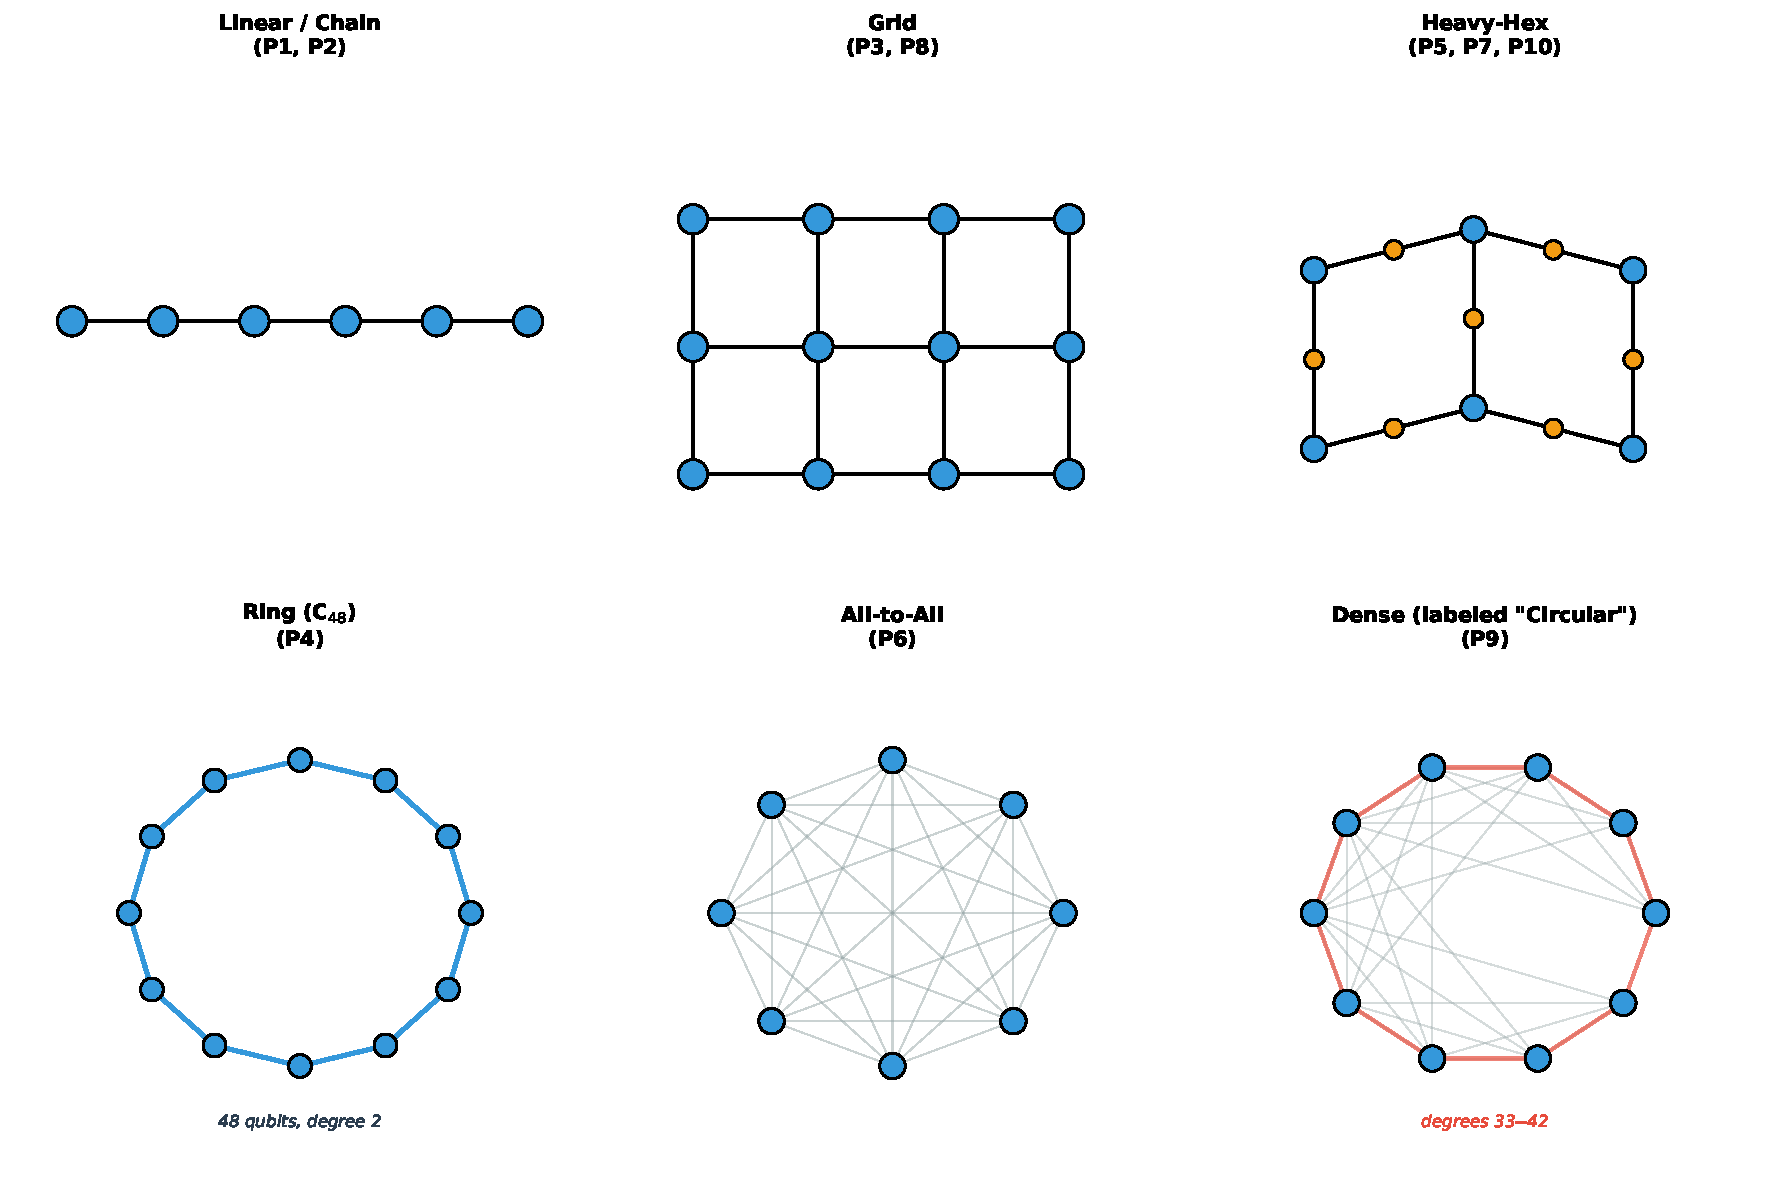
\includegraphics[width=\textwidth]{figures/fig2_topologies.pdf}
\caption{Coupling map topologies across the ten peaked circuits. Orange nodes in Heavy-Hex indicate bridge qubits. P9's dense connectivity (degrees 33--42) contradicts its ``Circular'' label.}
\label{fig:topologies}
\end{figure}

\subsection{Complexity Landscape}

Figure~\ref{fig:complexity} plots each circuit in the qubits--vs--two-qubit-gates space. The three solved circuits cluster in the low-gate-count region, while unsolved circuits occupy a distinct high-complexity regime.

\begin{figure}[H]
\centering
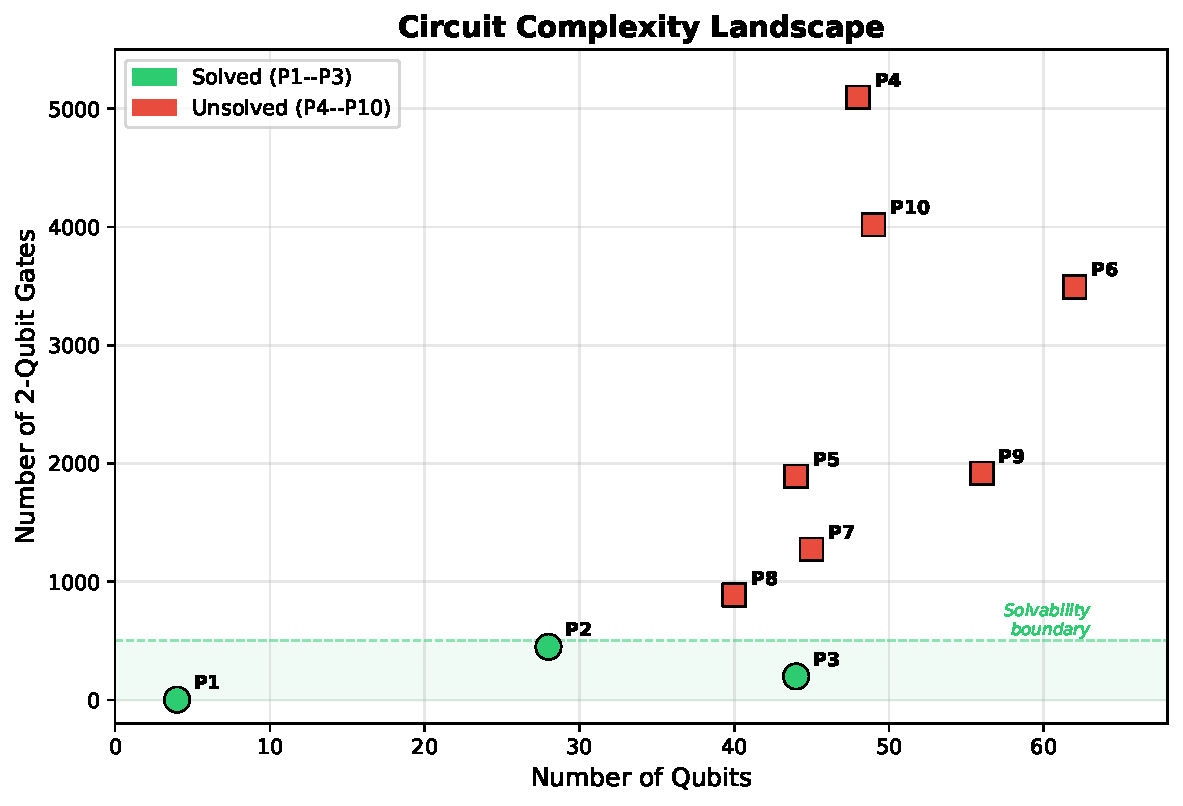
\includegraphics[width=0.75\textwidth]{figures/fig1_complexity.pdf}
\caption{Circuit complexity landscape. Solved circuits (green circles) have significantly fewer two-qubit gates than unsolved ones (red squares), regardless of qubit count.}
\label{fig:complexity}
\end{figure}

% ============================================================================
\section{Methods}
\label{sec:methods}

We employed eight distinct simulation strategies, escalating from exact classical methods to approximate tensor networks to real quantum hardware.

\subsection{Exact Statevector Simulation}
\label{sec:statevector}

For circuits with $n \leq 34$ qubits, exact statevector simulation is feasible, requiring $\bigO(2^n)$ memory. We used BlueQubit's cloud \texttt{cpu} device, which provides full statevector access.

\textbf{Results:}
\begin{itemize}[nosep]
    \item \circuit{P1} (4 qubits): Solved in 12\,ms. Peak bitstring \texttt{1001} with probability 66.93\%.
    \item \circuit{P2} (28 qubits): Solved in 29.2\,s. Peak bitstring \texttt{1100101101100011011000011100} with probability 34.88\%.
\end{itemize}

Both P1 and P2 had qubit counts within the statevector regime. P3 at 44 qubits would require $2^{44} \times 16$\,bytes $\approx 256$\,TB of memory, ruling out exact simulation.

\subsection{Matrix Product State Simulation}
\label{sec:mps}

Matrix product states~\cite{schollwock2011density,orus2014practical} represent an $n$-qubit state as a chain of tensors:
\begin{equation}
\ket{\psi} = \sum_{i_1,\ldots,i_n} A^{[1]}_{i_1} A^{[2]}_{i_2} \cdots A^{[n]}_{i_n} \ket{i_1 i_2 \cdots i_n}
\end{equation}
where each $A^{[k]}_{i_k}$ is a $\bd_{k-1} \times \bd_k$ matrix. The maximum bond dimension $\bd_{\max}$ controls the trade-off between accuracy and computational cost: simulation scales as $\bigO(n \cdot \bd_{\max}^3)$ per gate, with $\bigO(n \cdot \bd_{\max}^2)$ memory.

We used Qiskit Aer's MPS simulator~\cite{qiskit2024} (locally) and BlueQubit's cloud \texttt{mps.cpu} device with bond dimensions $\bd \in \{64, 128, 256, 512, 1024, 2048\}$.

\textbf{Results:}
\begin{itemize}[nosep]
    \item \circuit{P3} (44 qubits, grid): Solved at $\bd = 256$ via BlueQubit \texttt{mps.cpu} in 2.1\,minutes. Peak bitstring found with 11.01\% probability (1{,}101 of 10{,}000 shots).
    \item \circuit{P4--P10}: All bond dimensions up to $\bd = 1024$ (locally) and $\bd = 2048$ (cloud estimates) returned uniformly random outputs---10{,}000 unique bitstrings from 10{,}000 shots, each appearing exactly once.
\end{itemize}

Figure~\ref{fig:mps_scaling} shows the MPS runtime scaling for P4 (after RCM reordering) as a function of bond dimension. Despite super-polynomial growth in compute time, all runs produced noise.

\begin{figure}[H]
\centering
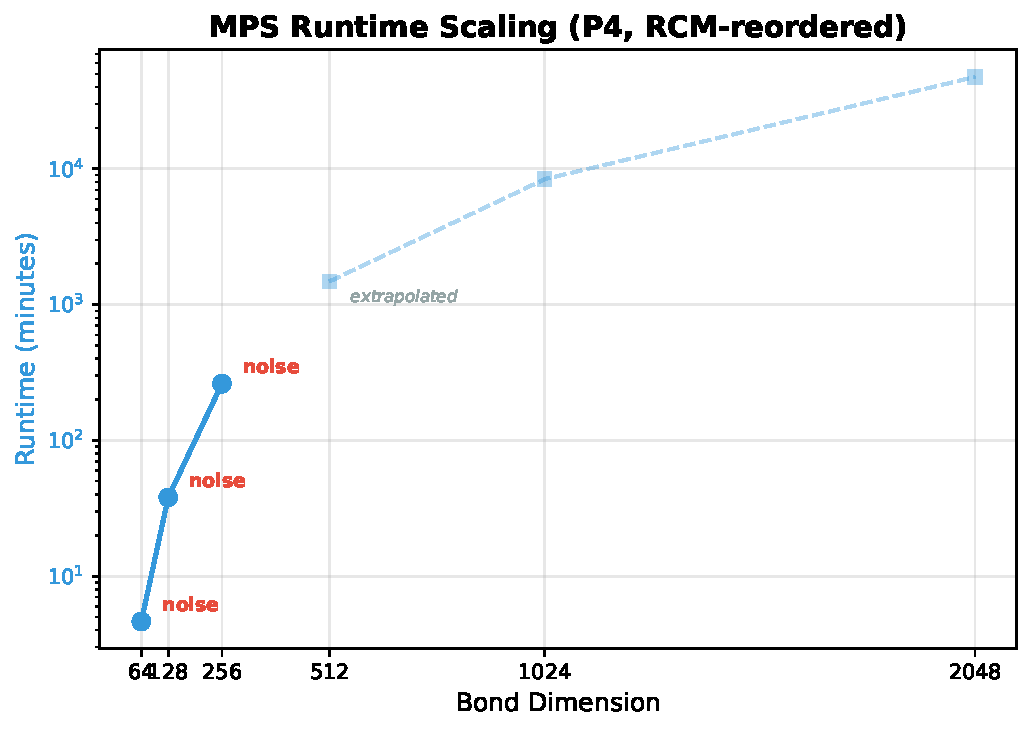
\includegraphics[width=0.75\textwidth]{figures/fig3_mps_scaling.pdf}
\caption{MPS runtime scaling for P4 (48 qubits, RCM-reordered). All bond dimensions returned noise (uniformly random outputs). Dashed line shows extrapolated scaling.}
\label{fig:mps_scaling}
\end{figure}

\subsection{Reverse Cuthill--McKee Qubit Reordering}
\label{sec:rcm}

MPS methods perform best when entanglement is local in the qubit ordering. The Reverse Cuthill--McKee (RCM) algorithm~\cite{cuthill1969reducing} reorders vertices of a sparse graph to minimize bandwidth, potentially improving MPS performance by reducing long-range entanglement in the tensor chain.

We applied RCM reordering to circuits P4--P10 using NetworkX's \texttt{reverse\_cuthill\_mckee\_ordering}. Figure~\ref{fig:rcm} shows the bandwidth reduction achieved.

\begin{figure}[H]
\centering
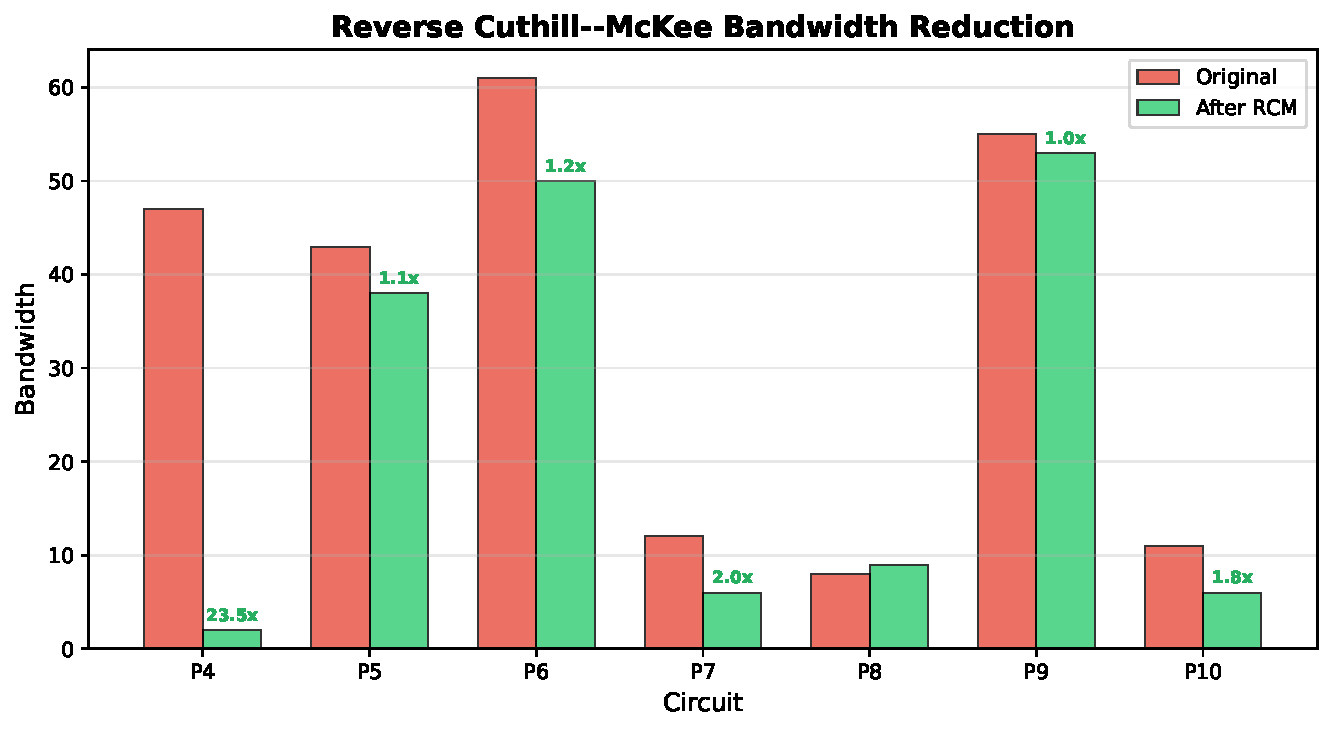
\includegraphics[width=0.8\textwidth]{figures/fig4_rcm_bandwidth.pdf}
\caption{Reverse Cuthill--McKee bandwidth reduction. P4 achieved a 23.5$\times$ improvement (bandwidth 47 $\to$ 2), effectively reducing the coupling graph to a nearly 1D chain. Dense topologies (P5, P6, P9) showed minimal improvement.}
\label{fig:rcm}
\end{figure}

\textbf{Key finding:} Despite reducing P4's bandwidth from 47 to 2 (making it effectively a 1D chain), the 5{,}096 CZ gates still generate entanglement that exceeds any computationally feasible bond dimension. At $\bd = 256$ after RCM reordering, the simulation took 4.4 hours and still returned noise. This demonstrates that gate \emph{depth}, not just topology, determines MPS tractability.

\subsection{Cloud Quantum Simulation}
\label{sec:cloud}

BlueQubit provides cloud-based simulation infrastructure with three device types:
\begin{itemize}[nosep]
    \item \texttt{mps.cpu}: CPU-based MPS simulation, free on subscription. Maximum $\bd = 2048$.
    \item \texttt{mps.gpu}: GPU-accelerated MPS, pay-per-use (\$10--17 per job at $\bd = 1024$).
    \item \texttt{tensor-network}: Full tensor network contraction (requires elevated authentication).
\end{itemize}

We submitted approximately 20 jobs to \texttt{mps.cpu} at bond dimensions 256--1024, with runtimes from 19.5 minutes (P8, $\bd = 256$) to an estimated 10.4 hours (P7, $\bd = 1024$). All completed jobs returned noise.

One GPU attempt (\texttt{mps.gpu}, P8, $\bd = 1024$, \$9.46) was terminated before completion. The \texttt{tensor-network} device returned an authorization error, and the \texttt{pauli-path} device computes expectation values rather than samples, making it unsuitable for peak-finding.

\subsection{Marginal Probability Reconstruction}
\label{sec:marginals}

We developed a marginal voting scheme to reconstruct the peak bitstring from noisy MPS outputs:
\begin{enumerate}[nosep]
    \item Run $R$ independent MPS simulations at low bond dimension with $S$ shots each.
    \item For each qubit $q$, compute the marginal probability $p_q = P(\text{qubit } q = 1)$ by aggregating across all runs.
    \item Reconstruct the candidate bitstring by majority vote: bit $q = 1$ if $p_q > 0.5$.
\end{enumerate}

\textbf{Results for P8 (40 qubits):}
\begin{itemize}[nosep]
    \item At $\bd = 64$: average confidence 0.627, only 17/40 qubits strongly determined ($|p_q - 0.5| > 0.1$). Runtime: 763\,s.
    \item At $\bd = 128$: average confidence 0.599 (worse), only 13/40 qubits strongly determined.
\end{itemize}

The decreasing confidence with increasing bond dimension suggests that at insufficient $\bd$, the MPS simulation produces structured noise that does not converge to the true marginals. The method fails because the underlying simulations themselves are inaccurate.

\subsection{Inverse Circuit Verification}
\label{sec:inverse}

Given a candidate bitstring $x$, we can verify correctness by constructing the circuit $X_x \cdot U^\dagger$ and checking whether it maps $\ket{0^n}$ to $\ket{0^n}$:
\begin{equation}
P(\text{all zeros}) = |\!\braket{0^n | U^\dagger X_x | 0^n}\!|^2 = |\!\braket{x | U | 0^n}\!|^2
\end{equation}
where $X_x$ applies Pauli-$X$ to qubits where $x$ has bit value 1. If $x$ is the peak bitstring, this probability should be significantly above $2^{-n}$.

We implemented this verification tool but could not deploy it effectively, as no simulation method produced plausible candidates to verify. The tool remains valuable for future work where approximate methods might generate near-correct bitstrings.

\subsection{Real Quantum Hardware}
\label{sec:hardware}

We executed circuits on two quantum hardware platforms:

\paragraph{IBM Quantum (ibm\_fez, Heron r2).}
IBM's 156-qubit Heron r2 processor~\cite{ibm2024heron} was used to run P5 (44 qubits, 1{,}892 CZ gates). After transpilation, the circuit exceeded the device's coherent operation window: all 10{,}000 shots returned unique bitstrings (pure noise), consistent with complete decoherence.

\paragraph{BlueQubit QPU.}
Attempts to run P7 and P8 on BlueQubit's quantum device were terminated because transpiled circuits exceeded the 20{,}000-gate limit (P7: 25{,}961 gates; P8: 29{,}729 gates after transpilation). Subsequent attempts for P5 and P9 failed due to insufficient account balance (\$31.60 available, \$37.20 required for four jobs at \$9.30 each).

\subsection{Alternative Tensor Network Methods}
\label{sec:quimb}

We attempted to use quimb~\cite{gray2018quimb} with the cotengra~\cite{gray2021hyper} contraction optimizer, which can exploit the full tensor network structure rather than restricting to an MPS decomposition. This approach is particularly promising for circuits with 2D or irregular topologies where tree tensor networks or PEPS representations may outperform MPS.

The attempt failed due to API incompatibility: quimb 1.12.1's \texttt{TensorNetworkGenVector} object lacked the expected \texttt{convert\_to\_mps} method. Additionally, cotengra operated without the recommended hyper-optimizers (kahypar, optuna) and fell back to random contraction order sampling, which is unlikely to find efficient contraction paths for circuits of this size.

% ============================================================================
\section{Results}
\label{sec:results}

\subsection{Solved Circuits}

Three circuits were successfully solved:
\begin{itemize}[nosep]
    \item \textbf{P1} (4 qubits, Linear): Bitstring \texttt{1001}, probability 66.93\%. Solved via exact statevector in 12\,ms.
    \item \textbf{P2} (28 qubits, Chain): Bitstring \texttt{1100101101100011011000011100}, probability 34.88\%. Solved via exact statevector in 29.2\,s.
    \item \textbf{P3} (44 qubits, Grid): Bitstring \texttt{10001101010101010000011111001101000100011010}, probability $\sim$11\%. Solved via MPS ($\bd = 256$) in 2.1\,min.
\end{itemize}

The solved circuits share two properties: (1) relatively few two-qubit gates ($\lesssim 450$) and (2) low-dimensional or sparse coupling topologies amenable to MPS.

\subsection{Failed Circuits}

Table~\ref{tab:attempts} summarizes the methods attempted for each unsolved circuit and the computational resources expended.

\begin{table}[H]
\centering
\caption{Summary of simulation attempts for unsolved circuits P4--P10. All attempts returned uniformly random (noise) outputs.}
\label{tab:attempts}
\small
\begin{tabularx}{\textwidth}{@{}lXl@{}}
\toprule
Circuit & Methods Attempted & Max Resources \\
\midrule
P4 (48q, 5096 CZ) & Local MPS $\bd$=64--256 with RCM; Cloud MPS & 4.4\,hr ($\bd$=256) \\
P5 (44q, 1892 CZ) & Cloud MPS $\bd$=256--1024; IBM QPU (ibm\_fez) & 15\,hr (est.) \\
P6 (62q, 3494 CZ) & Cloud MPS $\bd$=256--1024 & 10+\,hr (est.) \\
P7 (45q, 1275 CZ) & Cloud MPS $\bd$=256--1024; BQ QPU (terminated) & 10.4\,hr ($\bd$=1024) \\
P8 (40q, 888 iSwap) & Local MPS $\bd$=1024 (10+hr); Cloud MPS; GPU MPS; quimb & 10+\,hr local \\
P9 (56q, 1917 RZZ) & Cloud MPS; topology analysis & Pending \\
P10 (49q, 4020 CZ) & Cloud MPS & Pending \\
\bottomrule
\end{tabularx}
\end{table}

Figure~\ref{fig:results} provides a visual summary of all results.

\begin{figure}[H]
\centering
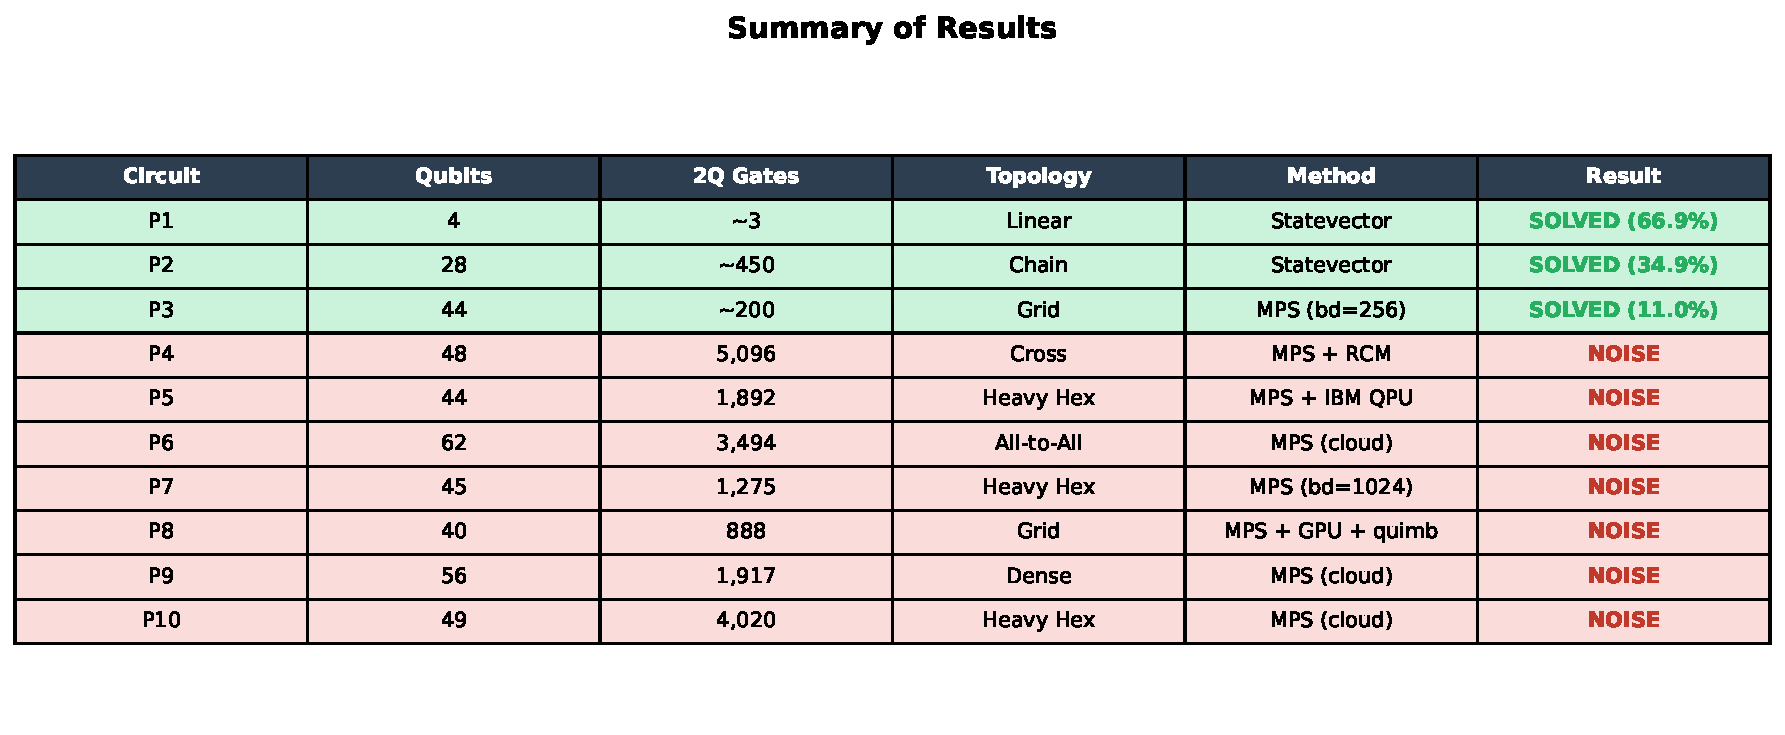
\includegraphics[width=\textwidth]{figures/fig5_results.pdf}
\caption{Summary of results across all ten peaked circuits. Green rows indicate successfully solved circuits; red rows indicate circuits where all simulation methods returned noise.}
\label{fig:results}
\end{figure}

% ============================================================================
\section{Discussion}
\label{sec:discussion}

\subsection{Why P4--P10 Failed}

The fundamental barrier is that circuits P4--P10 generate bipartite entanglement entropy that exceeds what MPS at any computationally feasible bond dimension can represent. For an MPS with bond dimension $\bd$, the maximum representable entanglement entropy across any bipartition is $S_{\max} = \log_2 \bd$. At $\bd = 1024$, this is only 10 ebits---far below what circuits with hundreds to thousands of entangling gates can produce.

Several factors compound this difficulty:
\begin{enumerate}[nosep]
    \item \textbf{Gate depth:} Even P8, the circuit with fewest two-qubit gates (888 iSWAP), generates sufficient entanglement to defeat $\bd = 1024$ MPS. The circuits are specifically designed to maximize entanglement.
    \item \textbf{Non-Clifford gates:} All circuits use non-Clifford gate sets (CZ, iSWAP, RZZ with non-Clifford angles), precluding efficient Clifford simulation via the Gottesman--Knill theorem~\cite{gottesman1998heisenberg}.
    \item \textbf{Dense topologies:} P6 (all-to-all) and P9 (degrees 33--42) have coupling maps where no qubit ordering achieves low MPS bandwidth, making tensor network methods inherently expensive.
    \item \textbf{Hardware limitations:} Current quantum processors lack the gate fidelity and coherence times to reliably execute circuits with thousands of two-qubit gates. IBM's Heron r2 processor produced pure noise on P5 (1{,}892 CZ gates).
\end{enumerate}

\subsection{Entanglement and Bond Dimension Requirements}

For a random quantum circuit on $n$ qubits with depth $d$, the entanglement entropy across a balanced bipartition grows as~\cite{nahum2017quantum}:
\begin{equation}
S(t) \approx \min\left(s_{\text{eq}} \cdot v_E \cdot t,\; \frac{n}{2}\right)
\end{equation}
where $v_E$ is the entanglement velocity and $s_{\text{eq}}$ is the equilibrium entropy density. For the unsolved circuits, even conservative estimates suggest $S > 15$--20 ebits, requiring $\bd > 2^{15} = 32{,}768$ to $2^{20} \approx 10^6$---far beyond current computational feasibility.

\subsection{Topology vs.\ Depth}

The RCM results for P4 provide a striking illustration: despite achieving near-optimal 1D ordering (bandwidth reduced from 47 to 2), the 5{,}096 CZ gates create a circuit deep enough that entanglement propagates through the entire chain multiple times. This demonstrates that \textbf{topology alone does not determine MPS tractability}---circuit depth is equally critical.

\subsection{The Marginal Reconstruction Failure}

The marginal voting approach failed because it relies on the assumption that low-$\bd$ MPS simulations produce outputs that are \emph{biased toward the correct answer}, even if individually noisy. Instead, we observed that insufficient bond dimension produces outputs indistinguishable from uniform random sampling. The per-qubit marginals converged to $p_q \approx 0.5$ (maximum entropy), providing no information about the true peak.

% ============================================================================
\section{Future Work}
\label{sec:future}

Several avenues remain unexplored that could potentially solve some of the remaining circuits:

\begin{enumerate}
    \item \textbf{GPU tensor network contraction:} Tools like cuTensorNet~\cite{nvidia2023cutensornet} on multi-GPU systems can contract tensor networks with significantly more memory and compute than CPU-based MPS. Combined with optimized contraction ordering (via cotengra with kahypar), this could handle circuits with moderate entanglement.

    \item \textbf{Circuit cutting:\!} Decomposing large circuits into smaller subcircuits that can be simulated independently, then combining results with classical post-processing~\cite{peng2020simulating}. The overhead scales exponentially with the number of cuts but may be feasible for sparse topologies like P4's cross pattern.

    \item \textbf{Variational methods:} Using a parameterized ansatz (e.g., variational MPS or MERA~\cite{vidal2007entanglement}) to directly optimize for the peak bitstring. The objective function $|\!\braket{x|U|0^n}\!|^2$ can be estimated via MPS contraction and optimized via gradient descent.

    \item \textbf{Error-mitigated quantum hardware:} Techniques such as zero-noise extrapolation, probabilistic error cancellation~\cite{temme2017error}, or tensor network error mitigation~\cite{filippov2023scalable} applied to noisy hardware results could extract signal from otherwise decoherent outputs.

    \item \textbf{Projected entangled pair states (PEPS):} For 2D topologies like P3 and P8, PEPS~\cite{verstraete2004renormalization} can represent states with area-law entanglement more efficiently than MPS. Approximate contraction algorithms exist but are computationally demanding.

    \item \textbf{Clifford + $T$ decomposition:} If the circuits can be decomposed into a Clifford backbone with few non-Clifford gates, stabilizer rank methods~\cite{bravyi2019simulation} could provide exponential speedup. However, the high non-Clifford gate counts likely preclude this approach.
\end{enumerate}

% ============================================================================
\section{Conclusions}
\label{sec:conclusions}

We systematically explored eight classical and quantum simulation methods for solving ten peaked quantum circuits in the BlueQubit ``Peaked Portal'' hackathon. Three circuits (P1--P3) were solved using exact statevector simulation and MPS methods. The remaining seven circuits (P4--P10) resisted all approaches, including MPS at bond dimensions up to 2{,}048, RCM-optimized qubit reordering, cloud GPU simulation, marginal probability reconstruction, real quantum hardware (IBM Heron r2), and alternative tensor network libraries.

The results underscore a key finding: \textbf{peaked circuits with $\gtrsim$\,888 two-qubit entangling gates on 40+ qubits generate entanglement that exceeds the representational capacity of current accessible simulation methods}. This boundary---between P3 (solvable, $\sim$200 two-qubit gates) and P8 (unsolvable, 888 two-qubit gates)---marks a practical frontier of classical simulability for this class of circuits.

Our work also highlights the gap between state-of-the-art quantum hardware and the requirements of these circuits. Even IBM's 156-qubit Heron r2 processor could not reliably execute a 44-qubit circuit with 1{,}892 CZ gates, producing pure decoherence noise. Bridging this gap---through improved hardware, better error mitigation, or more efficient classical algorithms---remains an open challenge at the intersection of quantum computing and computational complexity theory.

Figure~\ref{fig:flowchart} summarizes the decision strategy employed throughout this work.

\begin{figure}[H]
\centering
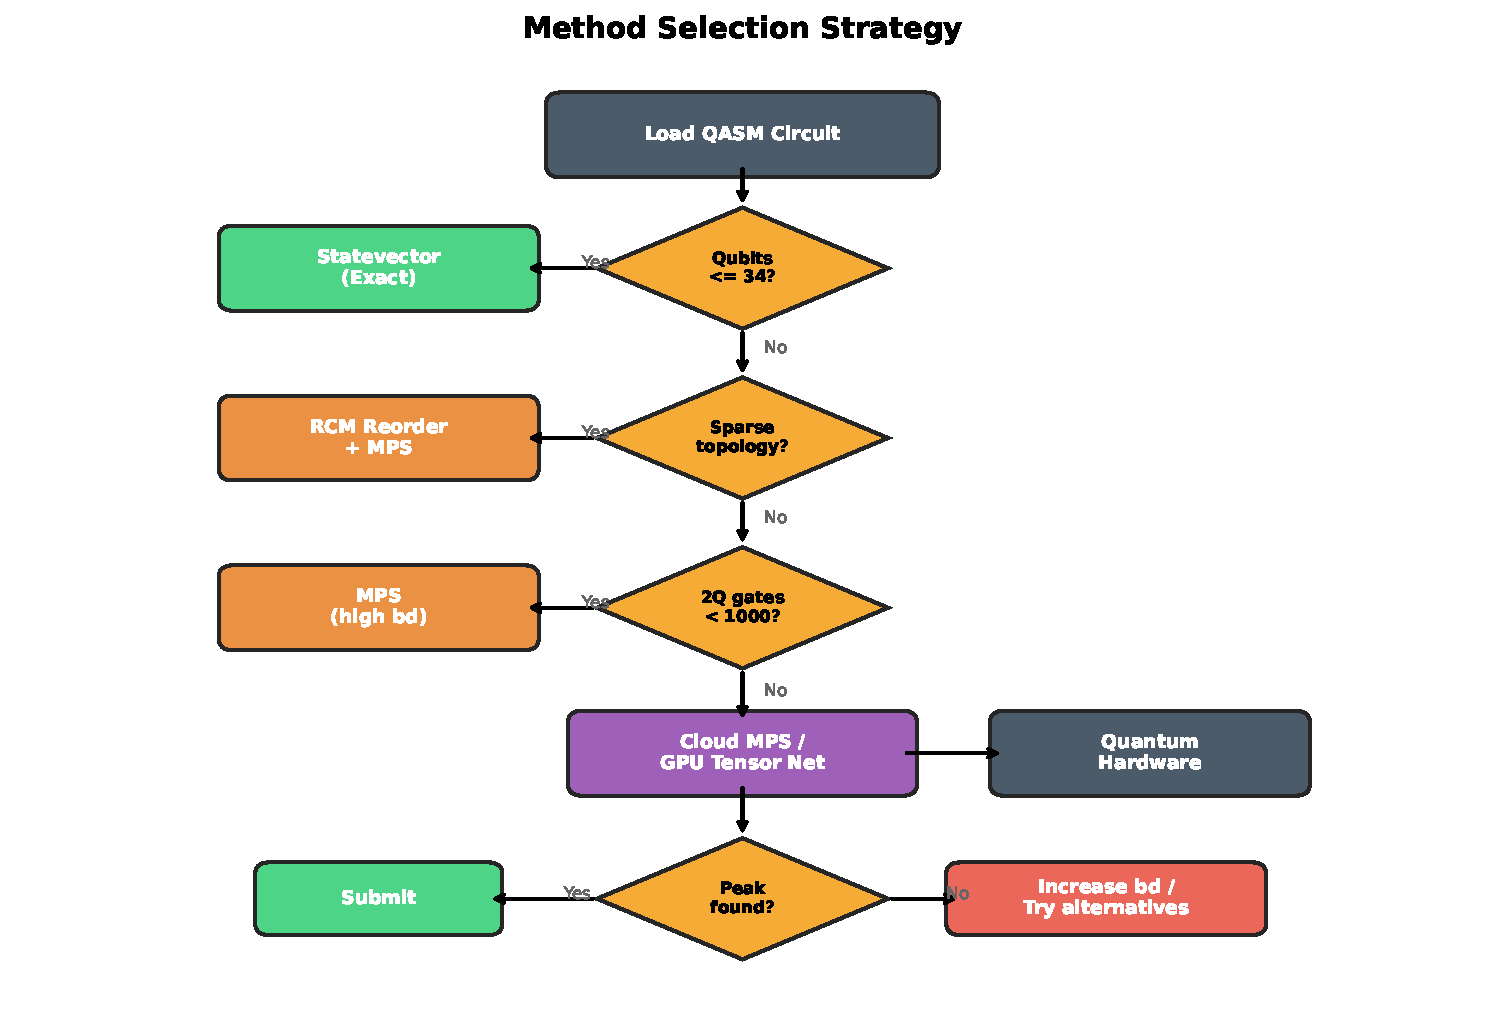
\includegraphics[width=0.85\textwidth]{figures/fig6_flowchart.pdf}
\caption{Method selection strategy employed during the hackathon. The flowchart illustrates the escalation from exact simulation through approximate classical methods to quantum hardware.}
\label{fig:flowchart}
\end{figure}

% ============================================================================
\bibliographystyle{unsrtnat}

\begin{thebibliography}{20}

\bibitem{arute2019quantum}
F.~Arute \emph{et al.},
``Quantum supremacy using a programmable superconducting processor,''
\emph{Nature}, vol.~574, pp.~505--510, 2019.

\bibitem{zhong2020quantum}
H.-S. Zhong \emph{et al.},
``Quantum computational advantage using photons,''
\emph{Science}, vol.~370, pp.~1460--1463, 2020.

\bibitem{aaronson2017complexity}
S.~Aaronson and L.~Chen,
``Complexity-theoretic foundations of quantum supremacy experiments,''
\emph{Proc.\ 32nd CCC}, pp.~22:1--22:67, 2017.

\bibitem{bluequbit2025hackathon}
BlueQubit,
``Peaked Portal Quantum Computing Hackathon,''
\url{https://www.bluequbit.io/quantum-computing-hackathon}, 2025.

\bibitem{schollwock2011density}
U.~Schollw{\"o}ck,
``The density-matrix renormalization group in the age of matrix product states,''
\emph{Ann.\ Phys.}, vol.~326, pp.~96--192, 2011.

\bibitem{orus2014practical}
R.~Or{\'u}s,
``A practical introduction to tensor networks: Matrix product states and projected entangled pair states,''
\emph{Ann.\ Phys.}, vol.~349, pp.~117--158, 2014.

\bibitem{qiskit2024}
Qiskit contributors,
``Qiskit: An open-source framework for quantum computing,''
\url{https://qiskit.org/}, 2024.

\bibitem{cuthill1969reducing}
E.~Cuthill and J.~McKee,
``Reducing the bandwidth of sparse symmetric matrices,''
\emph{Proc.\ 24th ACM Nat.\ Conf.}, pp.~157--172, 1969.

\bibitem{gottesman1998heisenberg}
D.~Gottesman,
``The Heisenberg representation of quantum computers,''
\emph{Proc.\ 22nd ICGTMP}, pp.~32--43, 1998.

\bibitem{nahum2017quantum}
A.~Nahum, J.~Ruhman, S.~Vijay, and J.~Haah,
``Quantum entanglement growth under random unitary dynamics,''
\emph{Phys.\ Rev.\ X}, vol.~7, p.~031016, 2017.

\bibitem{gray2018quimb}
J.~Gray,
``quimb: A Python library for quantum information and many-body calculations,''
\emph{J.\ Open Source Softw.}, vol.~3, p.~819, 2018.

\bibitem{gray2021hyper}
J.~Gray and S.~Kourtis,
``Hyper-optimized tensor network contraction,''
\emph{Quantum}, vol.~5, p.~410, 2021.

\bibitem{nvidia2023cutensornet}
NVIDIA,
``cuTensorNet: GPU-accelerated tensor network computations,''
\url{https://docs.nvidia.com/cuda/cuquantum/}, 2023.

\bibitem{peng2020simulating}
T.~Peng, A.~W.~Harrow, M.~Ozols, and X.~Wu,
``Simulating large quantum circuits on a small quantum computer,''
\emph{Phys.\ Rev.\ Lett.}, vol.~125, p.~150504, 2020.

\bibitem{vidal2007entanglement}
G.~Vidal,
``Entanglement renormalization,''
\emph{Phys.\ Rev.\ Lett.}, vol.~99, p.~220405, 2007.

\bibitem{temme2017error}
K.~Temme, S.~Bravyi, and J.~M.~Gambetta,
``Error mitigation for short-depth quantum circuits,''
\emph{Phys.\ Rev.\ Lett.}, vol.~119, p.~180509, 2017.

\bibitem{filippov2023scalable}
S.~N.~Filippov \emph{et al.},
``Scalable tensor-network error mitigation for near-term quantum computing,''
arXiv:2307.11740, 2023.

\bibitem{verstraete2004renormalization}
F.~Verstraete and J.~I.~Cirac,
``Renormalization algorithms for quantum-many body systems in two and higher dimensions,''
arXiv:cond-mat/0407066, 2004.

\bibitem{bravyi2019simulation}
S.~Bravyi, D.~Browne, P.~Calpin, E.~Campbell, D.~Gosset, and M.~Howard,
``Simulation of quantum circuits by low-rank stabilizer decompositions,''
\emph{Quantum}, vol.~3, p.~181, 2019.

\bibitem{ibm2024heron}
IBM Quantum,
``IBM Heron processor,''
\url{https://www.ibm.com/quantum/processors}, 2024.

\bibitem{hagberg2008exploring}
A.~A.~Hagberg, D.~A.~Schult, and P.~J.~Swart,
``Exploring network structure, dynamics, and function using NetworkX,''
\emph{Proc.\ 7th Python in Science Conf.}, pp.~11--15, 2008.

\end{thebibliography}

\end{document}
